\documentclass[11pt,a4paper]{article}

\usepackage{pifont}
\usepackage{amsmath}
\usepackage{amssymb}
\usepackage{psfig}
\usepackage{graphicx}
\usepackage{array}
\usepackage{fancyheadings}
\usepackage{here}
\usepackage{eepic,epic}
\usepackage[english]{babel}

\input{YRpersdf}

\oddsidemargin -0.9cm
\evensidemargin -0.9cm
\topmargin -1cm
\textheight 22.5cm
\textwidth 17.6cm
\headheight 1.0cm

% principal notations



\begin{document}

\begin{center}
  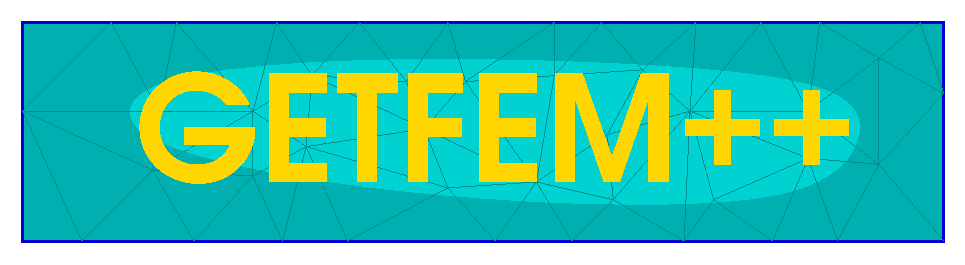
\includegraphics[width=10cm,angle=0]{getfem_logo.eps}\\[0.2cm]
  a Generic Finite Element library in C++ \\[0.5cm]
  \fbox{\Huge \sc Short User Documentation} \\[0.5cm]
  { \large Yves \sc Renard\footnote{ \it MIP, INSAT, Complexe scientifique de Rangueil, 31077 Toulouse, France, Yves.Renard@gmm.insa-tlse.fr } } \\[1.0cm]
  July 05, 2002\\[1.0cm]
\end{center}

% \begin{abstract}
% Basic user documentation for GETFEM++.
% \end{abstract}


%%%%%%%%%%%%%%%%%%%%%%%%%%%%%%%%%%%%%%%%%%%%%%%%%%%%%%%%%%%%%%%%%%%%%%%%%
%          INTRODUCTION                                                 %
%%%%%%%%%%%%%%%%%%%%%%%%%%%%%%%%%%%%%%%%%%%%%%%%%%%%%%%%%%%%%%%%%%%%%%%%%

\section*{Introduction}


The GETFEM++ project is centered around the development of a generic and efficient elementary computations C++ library for finite element methods. The goal is to build a library which allows to compute any elementary matrix (even for mixed methods) on the largest class of methods and elements and for arbitrary dimension. It offers a complete separation between integration methods (exact or approximated), geometric transformations (linear or not) and finite element methods of arbitrary degrees. It allows to write finite element code which are independent of the particular method, and thus to test easily various finite element method on the same problem.

 Moreover, the library includes other tools for computation with finite element such as assembling methods for classical PDEs, interpolation methods, computation of norms, mesh operations, boundary conditions ... This library allows to build finite elements codes which are completely independent of the dimension, the particular method or element. Examples are provided.\\[3cm]
Copyright (C) 2002\\
The program GETFEM++ is free software; you can redistribute it and/or modify
it under the terms of the GNU General Public License as published by
the Free Software Foundation; version 2 of the License.
This program is distributed in the hope that it will be useful,
but WITHOUT ANY WARRANTY; without even the implied warranty of
MERCHANTABILITY or FITNESS FOR A PARTICULAR PURPOSE.  See the
GNU General Public License for more details.
You should have received a copy of the GNU General Public License
along with this program; if not, write to the Free Software Foundation,
Inc., 59 Temple Place - Suite 330, Boston, MA  02111-1307, USA.

\newpage
\tableofcontents
\newpage

\section{Build a mesh}
GETFEM++ has it own structure to store meshes defined in the files {\tt bgeot\_mesh\_structure.h}, $\;$ ${\tt bgeot\_mesh.h}$ and {\tt getfem\_mesh.h}. The main structure is defined in {\tt getfem\_mesh.h} by the object\\[0.5cm]
{\tt getfem::getfem\_mesh }\\[0.5cm]
This object is able to store any element in any dimension even if you mix elements with different dimensions.\\[0.5cm]

There is no meshing procedures in GETFEM++ to mesh complex geometries. This is not the goal of this package. But you can easily load a mesh from any format.

\subsection{Add an element to a mesh}
Suppose the variable mesh has been declared by\\[0.5cm]
{\tt getfem::getfem\_mesh mesh;}\\[0.5cm]
then you have two ways to insert a new element to this mesh : from a list of points or from a list of indexes of already existing points.\\[0.5cm]
To enter a new point on a mesh use the method\\[0.5cm]
{\tt i = mesh.add\_point(pt);}\\[0.5cm]
where {\tt pt} is of type {\tt bgeot::base\_node}. The index {\tt i} is the index of this point on the mesh. If the point already exists in the mesh, a new point is not inserted and the index of the already existing point is returned. A mesh has a principal dimension, which is the dimension of its points. It is not possible to have points of different dimensions in a same mesh.\\[0.5cm]
The more basic function to add a new element to a mesh is\\[0.5cm]
{\tt j = mesh.add\_convex(pgt, it);}\\[0.5cm]
This is a template function, with {\tt pgt} of type {\tt bgeot::pgeometric\_trans} and {\tt it} is an iterator on a list of indexes of already existing points. For instance, if one needs to add a new triangle in a 3D mesh, one needs to define first an array with the indexes of the three points:\\[0.5cm]
{\tt 
  std::vector<bgeot::size\_type> ind(3); \\
  ind[0] = mesh.add\_point(bgeot::base\_node(0.0, 0.0, 0.0);\\
  ind[1] = mesh.add\_point(bgeot::base\_node(0.0, 1.0, 0.0);\\
  ind[2] = mesh.add\_point(bgeot::base\_node(0.0, 0.0, 1.0);
}\\[0.5cm]
then adding the element is done by\\[0.5cm]
{\tt mesh.add\_convex(bgeot::simplex\_trans(2,1), ind.begin()); }\\[0.5cm]
where {\tt mesh.add\_convex(bgeot::simplex\_trans(N,1);} denotes the usual linear geometric transformation for simplexes of dimension N.\\[0.5cm]
For simplexes, a more specialized function exists, which is\\[0.5cm]
{\tt mesh.add\_simplex(2, ind.begin()); }\\[0.5cm]

It is also possible to give directly the list of points with the function\\[0.5cm]
{\tt mesh.add\_convex\_by\_points(pgt, itp); }\\[0.5cm]
where now {\tt itp} is an iterator on an array of points. For example\\[0.5cm]
{\tt
  std::vector<bgeot::base\_node> pts(3); \\
  pts[0] = bgeot::base\_node(0.0, 0.0, 0.0); \\
  pts[0] = bgeot::base\_node(0.0, 1.0, 0.0); \\
  pts[0] = bgeot::base\_node(0.0, 0.0, 1.0); \\
  mesh.add\_convex\_by\_points(bgeot::simplex\_trans(2,1), pts.begin());
}\\[0.5cm]
Still add a triangle to the mesh.
It is possible to use also \\[0.5cm]
{\tt mesh.add\_simplex\_by\_points(2, pts.begin()); } \\[0.5cm]

For other elements than simplexes, it is still possible to use {\tt mesh.add\_convex\_by\_points} or $\ $$\ $ {\tt mesh.add\_convex} with the appropriate geometric transformation. \\[0.5cm]
{\tt bgeot::parallelepiped\_trans(N, 1) }
describes the usual transformation for parallelepipeds of dimension {\tt N} (quadrilateron for {\tt N=2}, hexahedron for {\tt N=3}, ...) \\[0.5cm]
{\tt bgeot::prism\_trans(N, 1) } 
describes the usual transformation for prisms of dimension {\tt N} (usual prism is for {\tt N=3}. A generalized prism is the product of a simplex of dimension {\tt N-1} with a segment) \\[0.5cm]
Specialized functions exist also: \\[0.5cm]
{\tt 
  mesh.add\_parallelepiped(N, it); \\
  mesh.add\_parallelepiped\_by\_points(N, itp); \\
  mesh.add\_prism(N, it); \\
  mesh.add\_prism\_by\_points(N, itp);
} \\[0.5cm]

The order of the points in the array of point is not important for simplexes. For other element, it is important to respect the order shown in figure \ref{fig:elem}.

\begin{figure}[htb] \label{fig:elem}
  \begin{center}
    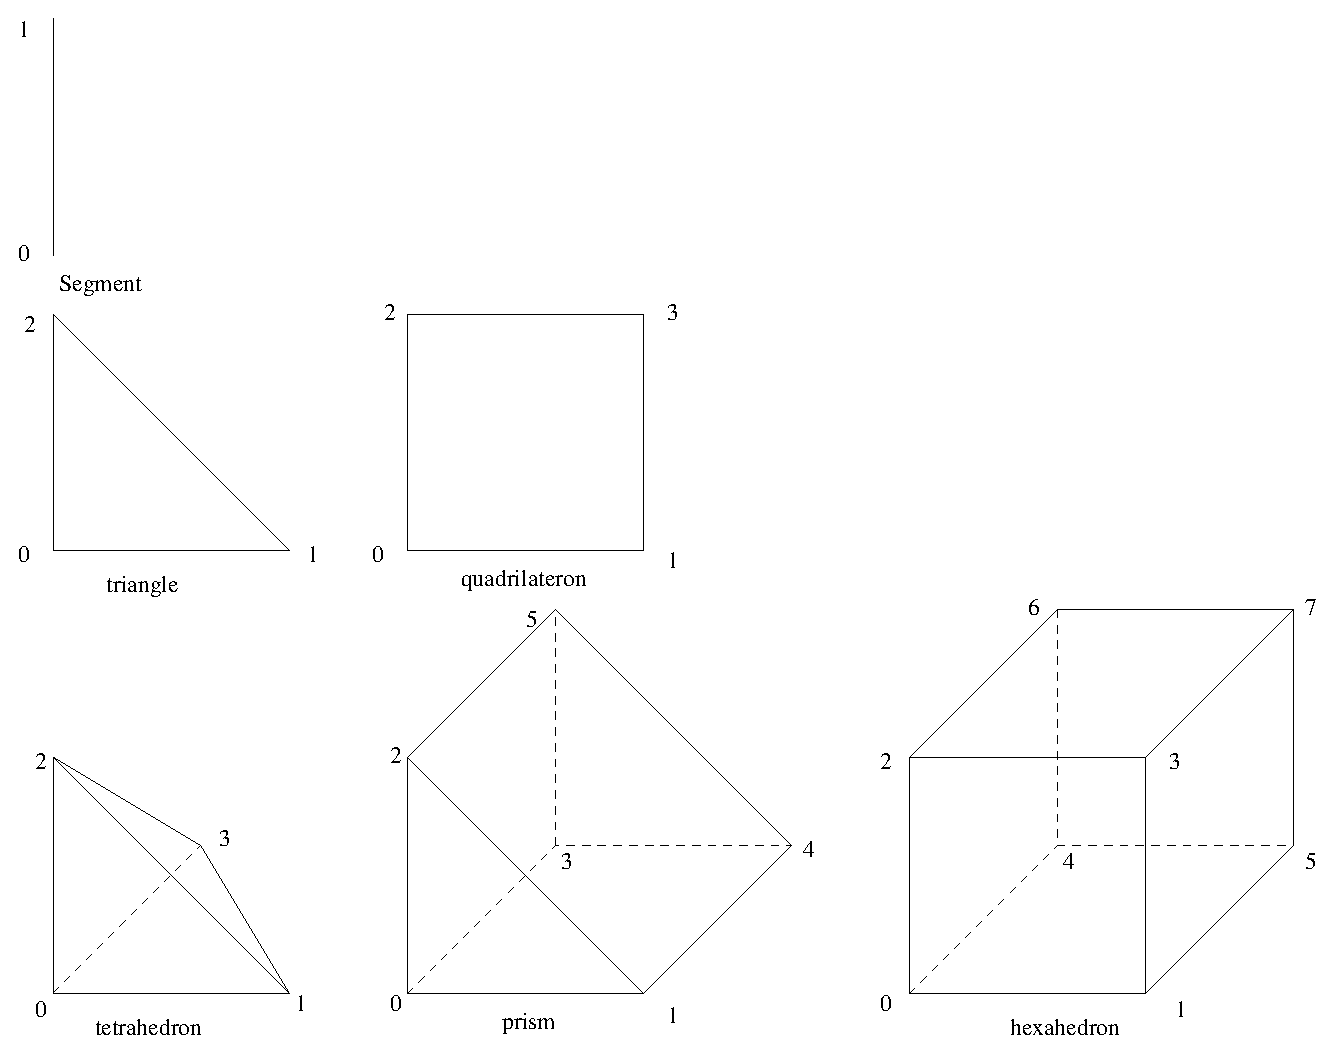
\includegraphics[width=15cm,angle=0]{getfemuser_elem.eps}
  \end{center}
  \caption{ \it vertex numeration for usual elements }
\end{figure}

\subsection{Remove an element from a mesh}
To remove an element from a mesh, simply use\\[0.5cm]
{\tt mesh.sup\_convex(i); }\\[0.5cm]
where {\tt i} is the index of the element.

\subsection{Simple structured meshes}

For parallelepiped domains, it is possible to obtain structured meshes with simplexes, parallelepipeds or prisms elements from three functions defined in {\tt getfem\_regular\_meshes.h}. \\[0.5cm]
{\tt
  getfem::parallelepiped\_regular\_simplex\_mesh(mesh, N, org, ivect, iref); \\
  getfem::parallelepiped\_regular\_prism\_mesh(mesh, N, org, ivect, iref); \\
  getfem::parallelepiped\_regular\_mesh(mesh, N, org, ivect, iref);
} \\[0.5cm]
where {\tt mesh} is a mesh variable in which the structured mesh will be built, {\tt N} is the dimension (limited to 4 for simplexes, 5 for prisms, unlimited for parallelepipeds), {\tt org} is of type {\tt bgeot::base\_node} and represents the origin of the mesh, {\tt ivect} is an iterator on an array of {\tt N} vectors to build the parallelepiped domain, {\tt iref} is an iterator on an array of {\tt N} integers representing the number of division on each direction. \\[0.5cm]
For instance, to build a mesh with tetrahedrons for a unit cube with $10\times10\times10$ cells one can write\\[0.5cm]
{\tt
  getfem::getfem\_mesh mesh; \\
  bgeot::base\_node org(0.0, 0.0, 0.0); \\
  std::vector<bgeot::base\_vector> vect(3); \\
  vect[0] = bgeot::base\_vector(1.0, 0.0, 0.0); \\
  vect[1] = bgeot::base\_vector(0.0, 1.0, 0.0); \\
  vect[2] = bgeot::base\_vector(0.0, 0.0, 1.0); \\
  std::vector<int> ref(3); \\
  ref[0] = ref[1] = ref[2] = 10; \\
  getfem::parallelepiped\_regular\_simplex\_mesh(mesh, 3, org, vect.begin(), ref.begin()); 
}\\[0.5cm]


\subsection{How to get information from a mesh}

Here is a list of functions to get information from an existing mesh. The list is not exhaustive.

\begin{center} \begin{tabular}{|m{0.4\linewidth}|m{0.55\linewidth}|} \hline

  {\tt mesh.dim()} & main dimension of the mesh.  \\ \hline

  {\tt mesh.points\_index()} & gives a {\tt dal::bit\_vector} object which represents all the indexes of valid points of a mesh (see in the following)  \\ \hline

  {\tt mesh.points()[i]} & gives the point of index {\tt i} (a {\tt bgeot::base\_node} ). \\ \hline
  
  {\tt mesh.convex\_index()} & gives a {\tt dal::bit\_vector} object which represents all the indexes of valid elements of a mesh (see in the following) \\ \hline

  {\tt mesh.structure\_of\_convex(i)} & gives the description of the structure of element of index {\tt i}. The function return a {\tt bgeot::pconvex\_structure}. \\ \hline

  {\tt mesh.structure\_of\_convex(i) ->nb\_faces()} & number of faces of  element of index {\tt i}. \\ \hline

  {\tt mesh.structure\_of\_convex(i) ->nb\_points()} & number of vertices of  element of index {\tt i}. \\ \hline

  {\tt mesh.structure\_of\_convex(i)->dim()} & intrinsic dimension of element of index {\tt i}. \\ \hline

  {\tt mesh.structure\_of\_convex(i) ->nb\_points\_of\_face(f)} & number of vertices of the face of local index {\tt f} of  element of index {\tt i}.\\ \hline
 
  {\tt mesh.structure\_of\_convex(i) ->ind\_points\_of\_face(f)} & return a container with the local indexes of all vertices of the face of local index {\tt f} of  element of index {\tt i}. For instance {\tt mesh.structure\_of\_convex(i) ->ind\_points\_of\_face(f)[0]} is the local index of the first vertex. \\ \hline

  {\tt mesh.structure\_of\_convex(i) ->face\_structure(f)} & gives the structure (a {\tt bgeot::pconvex\_structure}) of local index {\tt f} of  element of index {\tt i}.\\ \hline

  {\tt mesh.ind\_points\_of\_convex(i)} & gives a container with the global indexes of  vertices of element of index {\tt i}.\\ \hline

\end{tabular}
\begin{tabular}{|m{0.4\linewidth}|m{0.55\linewidth}|}\hline

  {\tt mesh.points\_of\_convex(i)} & gives a container with the  vertices of element of index {\tt i}. This is an array of {\tt bgeot::base\_node}.\\ \hline

  {\tt mesh.convex\_to\_point(ipt)} & gives a container with the indexes of all elements attached to the point of global index {\tt ipt}.\\ \hline

  {\tt convex\_with\_points(mesh, nb, ipts) } & gives a container with the indexes of all elements in {\tt mesh} having a certain set of points for vertices. The set of points is describe by an iterator {\tt ipts} on an array and the number of points {\tt nb}.\\ \hline

  {\tt neighbour\_of\_convex(mesh, ic, f)} & gives a container with the indexes of all elements in {\tt mesh} having the common face of local index {\tt f} of element {\tt ic} except element {\tt ic}. \\ \hline

  {\tt mesh.stat()} & print in {\tt std::cout} main information on the mesh. \\ \hline

  {\tt mesh.clear()} & delete all elements and points from the mesh. \\ \hline

  {\tt mesh.optimize\_structure()} & compact the structure. \\ \hline

  {\tt mesh.trans\_of\_convex(i)} & geometric transformation of the element of index {\tt i}. return a {\tt bgeot::pgeometric\_trans} (see \cite{BAS_COMP} for more details).  \\ \hline

  {\tt mesh.normal\_of\_face\_of\_convex(ic, f, pt)} & gives a {\tt bgeot::base\_vector} representing an outward normal to the element at the face of local index {\tt f} at the point of local coordinates (coordinates in the element of reference) {\tt pt}. The point {\tt pt} has no influence if the geometric transformation is linear. This is not a unit normal, the norm of the resulting vector is the ratio between the surface of the face of the reference element and the the surface of the face of the real element. \\ \hline

\end{tabular} \end{center}

About the object {\tt dal::bit\_vector}, which is very close to {\tt std::bit\_vector} but with additional functionalities to represent a set of non negative integers. If {\tt nn} is declared to be a {\tt dal::bit\_vector}, the two instructions {\tt nn.add(6)} or {\tt nn[6] = true} are equivalent and means that integer 6 is added to the set. In a same way {\tt nn.sup(6)} or {\tt nn[6] = false} remove the integer 6 from the set. The instruction {\tt nn.add(6, 10)} add the whole interval from 6 to 10 to the set (i.e. here 6, 7, 8, 9 and 10). To iterate on a {\tt dal::bit\_vector}, it is possible to use iterators as usual,  but, most of the time, as this object represents a set of integer, one just wants to iterate on the integers included into the set. This is possible with the operator \\[0.5cm]
{\tt i << nn; } \\[0.5cm]
This operator takes the first index such that {\tt nn[i] == true} and remove it (it makes nn[i] = false). If {\tt nn} is empty, the returned value for {\tt i} is -1. For instance, here is the code to iterate on the points of a mesh and print it to the standard output \\[0.5cm]
{\tt
  dal::bit\_vector nn = mesh.points\_index(); \\
  bgeot::size\_type i; \\
  for (i << nn; i != bgeot::size\_type(-1); i << nn) \\
  \mbox{}\hspace{1em}  cout << "Point of index " << i << " of the mesh : " << mesh.points()[i] << endl; \\
} \\[0.5cm]
The numeration of faces on usual elements is given in figure \ref{fig:elemf}.
\begin{figure}[htb] \label{fig:elemf}
  \begin{center}
    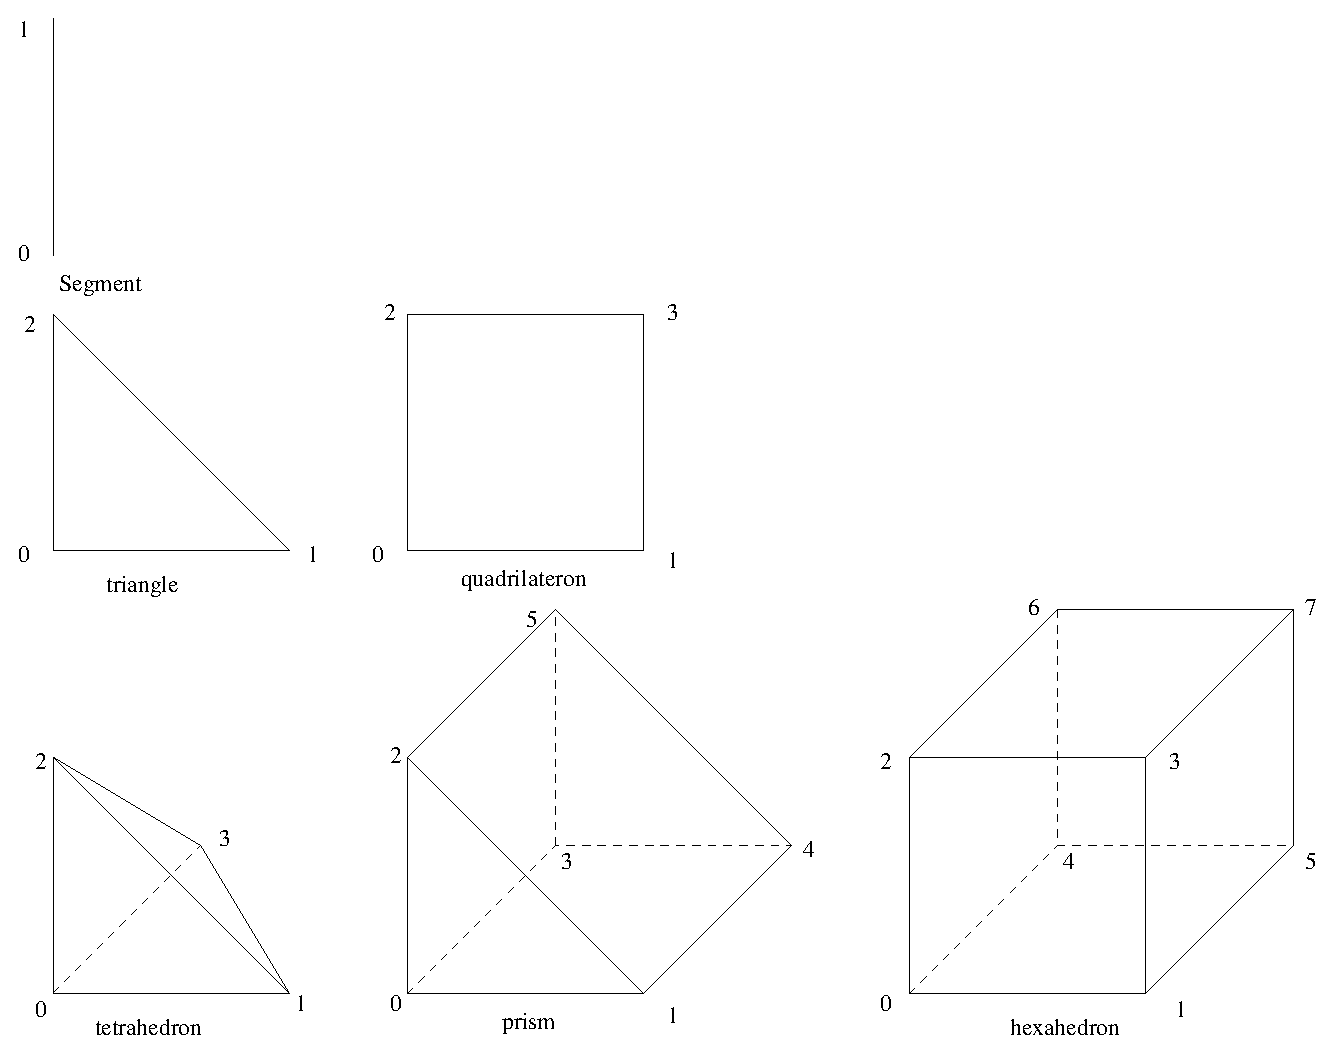
\includegraphics[width=15cm,angle=0]{getfemuser_elemf.eps}
  \end{center}
  \caption{ \it faces numeration for usual elements }
\end{figure}

\subsection{Save, load and draw meshes}

In {\tt getfem\_mesh.h}, two methods are defined to load meshes from file and write meshes to a file. \\[0.5cm]
\begin{tabular}{|m{0.4\linewidth}|m{0.55\linewidth}|}\hline

  {\tt mesh.write\_to\_file(const std::string \&name)} & save the mesh into a file.\\ \hline

  {\tt mesh.read\_from\_file(const std::string \&name)} & load the mesh from a file.\\ \hline

\end{tabular} \\[0.5cm]
At this stage of development, the loading function only accepts to load classical elements (simplexes, prisms and parallelepipeds with usual geometric transformations). If one needs other kind of elements, the loading function has to be extended.  \\[0.5cm]

A little tool allows to display a mesh using Gnuplot (and Perl). This tool is present in the directory {\tt contrib/} and of course you need to have a working distribution of Gnuplot installed on your system. This little tool is built when you execute a {\tt make} instruction on the root directory of GETFEM++. So, if GETFEM++ is normally installed on your system, you can change your current directory to {\tt contrib/} and execute the command \\[0.5cm]
{\tt draw\_mesh filename.mesh} \\[0.5cm]
where {\tt filename.mesh} is the file containing the mesh. This works only for meshes whose principal dimension is between 1 and 3. Examples of mesh files are also provided into the directory {\tt contrib/} to test the program.

\subsection{example}

The following is an example of how to load a mesh and extract information on it. \\[0.5cm]
{\tt
  \#include <getfem\_mesh.h> \\
  \\
  getfem::getfem\_mesh mesh; \\
  \\
  int main(int argc, char *argv[]) \{ \\
    $\mbox{}\ \ $ try \{ \\
    $\mbox{}\ \ \ \ $ \\
    $\mbox{}\ \ \ \ $ // read the mesh from the file name given by the first argument \\
    $\mbox{}\ \ \ \ $ mesh.read\_from\_file(std::string(argv[0])); \\
    $\mbox{}\ \ \ \ $ \\
    $\mbox{}\ \ \ \ $ // List all the convexes\\
    $\mbox{}\ \ \ \ $ dal::bit\_vector nn = mesh.convex\_index(); \\
    $\mbox{}\ \ \ \ $ bgeot::size\_type i; \\
    $\mbox{}\ \ \ \ $ for (i << nn; i != bgeot::size\_type(-1); i << nn) \{\\
    $\mbox{}\ \ \ \ \ \ $ cout << "Convex of index " << i << endl; \\
    $\mbox{}\ \ \ \ \ \ $ bgeot::pconvex\_structure cvs =  mesh.structure\_of\_convex(i); \\
    $\mbox{}\ \ \ \ \ \ $ cout << "Number of vertices : " << cvs->nb\_points() << endl; \\
    $\mbox{}\ \ \ \ \ \ $ cout << "Number of faces : " << cvs->nb\_faces() << endl;\\
    $\mbox{}\ \ \ \ \ \ $ for (bgeot::size\_type f = 0; f < cvs->nb\_faces(); ++f) \{\\
    $\mbox{}\ \ \ \ \ \ \ \ $ cout << "face " << f << " has " << cvs->nb\_points\_of\_face(f); \\
    $\mbox{}\ \ \ \ \ \ \ \ $ cout << " vertices with local indexes : "; \\
    $\mbox{}\ \ \ \ \ \ \ \ $ for (bgeot::size\_type k = 0; k < cvs->nb\_points\_of\_face(f); ++k) \\
    $\mbox{}\ \ \ \ \ \ \ \ \ \ $ cout << cvs->ind\_points\_of\_face(f)[k] << " "; \\ 
    $\mbox{}\ \ \ \ \ \ \ \ $ cout << " and global indexes : ";\\
    $\mbox{}\ \ \ \ \ \ \ \ $ for (bgeot::size\_type k = 0; k < cvs->nb\_points\_of\_face(f); ++k) \\
    $\mbox{}\ \ \ \ \ \ \ \ \ \ $ cout << mesh.ind\_points\_of\_convex(i)(cvs->ind\_points\_of\_face(f)[k]) << " "; \\ 
    $\mbox{}\ \ \ \ \ \ \}$ \\
    $\mbox{}\ \ \ \ \}$ \\
    $\mbox{}\ \ $ \} DAL\_STANDARD\_CATCH\_ERROR; // catches standard errors\\
  \}

}

\section{Select finite element and integration methods}

In order to define a complete finite element procedure on a mesh, the structure {\tt getfem::mesh\_fem} is defined in the file {\tt getfem\_mesh\_fem.h}. Basically, this structure describe the finite element method on each element of the mesh, and can store information about boundary structure. It is possible to have an arbitrary number of finite element description for a single mesh. This is particularly necessary for mixed methods, but also to describe different data on the same mesh. One can instantiate a {\tt getfem::mesh\_fem} object as follows\\[0.5cm]
{\tt getfem::mesh\_fem mef(mesh); }\\[0.5cm]
where {\tt mesh} is an already existing mesh. The structure will be linked to this mesh and will react when modifications will be done on it. \\[0.5cm]
It is possible to specify element by element the finite element method, so that element of mixed types can be treated, even if the dimensions are different. For usual elements, the connection between two elements is done when the two elements are compatibles (same degrees of freedom on the common face). A numeration of the degrees of freedom is automatically done with a Cuthill Mc Kee like algorithm. You have to keep in mind that there is absolutely no connection between the numeration of vertices of the mesh and the numeration of the degrees of freedom. Every {\tt getfem::mesh\_fem} object has its own numeration. \\[0.5cm]
To select a particular finite element method on a given element, one can use \\[0.5cm]
{\tt mef.set\_finite\_element(i, ppf, ppi); }\\[0.5cm]
where {\tt i} is the index of the element, {\tt ppf} is the descriptor of the finite element method, and {\tt ppi} is the descriptor of the integration method. The list of all available descriptors of finite element methods is in the file {\tt getfem\_fem.h}. A short description is also given in \cite{BAS_COMP}. The list of all available descriptors of integration methods is in the file {\tt bgeot\_poly\_integration.h} for exact integration methods and in the file {\tt bgeot\_approx\_integration.h} for approximate integration methods. \\[0.5cm]
A non exhautive list of finite element methods is given by
\begin{center} \begin{tabular}{|m{0.55\linewidth}|m{0.4\linewidth}|} \hline
{\tt getfem::ppolyfem getfem::PK\_fem(n, k)} & Classical $P_K$ methods on simplexes of dimension  {\tt n} with degree {\tt k} polynomials.\\ \hline
{\tt getfem::ppolyfem getfem::QK\_fem(n, k)} & Classical $Q_K$ methods on parallelepiped of dimension {\tt n}. Tensorial product of degree {\tt k} $P_K$ method on the segment. \\ \hline
{\tt getfem::ppolyfem getfem::PK\_prism\_fem(n, k)} & Classical methods on prism of dimension {\tt n}. Tensorial product of two degree {\tt k} $P_K$ method. \\ \hline
{\tt getfem::ppolyfem getfem::product\_fem( ppolyfem\;a, ppolyfem b)} & Tensorial product of the two polynomial finite element method {\tt a} and {\tt b}. \\ \hline
{\tt getfem::ppolyfem $\;$ getfem::P1\_nonconforming\_fem()} & Non conforming $P_1$ method on triangles. \\ \hline
\end{tabular} \end{center}

A list of exact integration methods is given by
\begin{center} \begin{tabular}{|m{0.55\linewidth}|m{0.4\linewidth}|} \hline
{\tt "IM\_EXACT\_SIMPLEX(n)"} & Description of the exact integration of polynomials on the simplex of reference of dimension {\tt n}. \\ \hline
\end{tabular}  
\begin{tabular}{|m{0.55\linewidth}|m{0.4\linewidth}|} \hline
{\tt "IM\_PRODUCT(a, b)"} & Description of the exact integration on the convex which is the direct product of the convex in {\tt a} and in {\tt b}.\\ \hline
\end{tabular}  
\begin{tabular}{|m{0.55\linewidth}|m{0.4\linewidth}|} \hline
{\tt "IM\_EXACT\_PARALLELEPIPED(n)"} & Description of the exact integration of polynomials on the parallelepiped of reference of dimension {\tt n}\\ \hline
\end{tabular}  
\begin{tabular}{|m{0.55\linewidth}|m{0.4\linewidth}|} \hline
{\tt "IM\_EXACT\_PRISM(n)"} & Description of the exact integration of polynomials on the prism of reference of dimension {\tt n}\\ \hline
\end{tabular} \end{center}

A list of approximated integration methods is given by
\begin{center} \begin{tabular}{|m{0.55\linewidth}|m{0.4\linewidth}|} \hline
{\tt "IM\_GAUSS1D(k)" } & Description of the Gauss integration on a segment of order {\tt k}. \\ \hline
\end{tabular}  
\begin{tabular}{|m{0.55\linewidth}|m{0.4\linewidth}|} \hline
{\tt "IM\_NC(n,k)"} & Description of the integration on a simplex of reference of dimension {\tt n} for polynomials of degree {\tt k} with the Newton Cotes method (based on Lagrange interpolation).\\ \hline
\end{tabular}  
\begin{tabular}{|m{0.55\linewidth}|m{0.4\linewidth}|} \hline
{\tt "IM\_PRODUCT(a,b)"} & Build a method doing the direct product of methods {\tt a} and {\tt b}. \\ \hline
\end{tabular}  
\begin{tabular}{|m{0.55\linewidth}|m{0.4\linewidth}|} \hline
{\tt "IM\_TRIANGLE(2)"} & Integration on a triangle of order 2 with 3 points. \\ \hline
\end{tabular}
\begin{tabular}{|m{0.55\linewidth}|m{0.4\linewidth}|} \hline
{\tt "IM\_TRIANGLE(7)"} & Integration on a triangle of order 7 with 13 points. \\ \hline
\end{tabular} 
\begin{tabular}{|m{0.55\linewidth}|m{0.4\linewidth}|} \hline
{\tt "IM\_QUAD(2)"} & Integration on quadrilaterals of order 2 with 3 points. \\ \hline
\end{tabular}
\begin{tabular}{|m{0.55\linewidth}|m{0.4\linewidth}|} \hline
{\tt "IM\_TETRAHEDRON(5)"} & Integration on a tetrahedron of order 5 with 15 points. \\ \hline
\end{tabular} \end{center}


For instance if one needs to have a description of a $P_1$ finite element method on a triangle with an exact integration, the way to set it is\\[0.5cm]
{\tt mef.set\_finite\_element(i, getfem::PK\_fem(2, 1), bgeot::simplex\_poly\_integration(2)); }\\[0.5cm]
where {\tt i} is still the index of the triangle. It is also possible to select a particular method directly on a set of element, passing to {\tt mef.set\_finite\_element} a {\tt dal::bit\_vector} instead of a single index. For instance\\[0.5cm]
{\tt mef.set\_finite\_element(mesh.convex\_index(), getfem::PK\_fem(2, 1),\\$\mbox{}\ \ \ \ \ \ \ \ \ \ \ \ \ \ \ \ \ \ \ \ \ \ $ bgeot::simplex\_poly\_integration(2)); }\\[0.5cm]
select the method on all the elements of the mesh.

Once a finite element method is defined on a mesh, it is possible to obtain information on it with the following methods (the list is not exhaustive).\\[0.5cm]
\begin{center} \begin{tabular}{|m{0.4\linewidth}|m{0.55\linewidth}|} \hline

  {\tt mef.convex\_index()} & Set of indexes (a {\tt dal::bit\_vector}) on which a finite element method is defined.  \\ \hline

  {\tt mef.linked\_mesh()} & gives a reference to the linked mesh.  \\ \hline

  {\tt mef.fem\_of\_element(i)} & gives a descriptor on the finite element method defined on element of index {\tt i}.  \\ \hline

  {\tt mef.int\_method\_of\_element(i)} & gives a descriptor on the integration method defined on element of index {\tt i}.  \\ \hline

  {\tt mef.nb\_dof\_of\_element(i)} & gives the number of degrees of freedom on the element of index {\tt i}.  \\ \hline

  {\tt mef.ind\_dof\_of\_element(i)} & gives a container (an array) with all the global indexes of the degrees of freedom of element of index {\tt i}.  \\ \hline

  {\tt mef.point\_of\_dof(i, j)} & gives a {\tt bgeot::base\_node} which represents the point associated with the dof of local index {\tt j} on element of index {\tt i}.  \\ \hline

  {\tt mef.point\_of\_dof(j)} & gives a {\tt bgeot::base\_node} which represents the point associated with the dof of global index {\tt j}.  \\ \hline

  {\tt mef.reference\_point\_of\_dof(i, j)} & gives a {\tt bgeot::base\_node} which represents the point associated with the dof of local index {\tt j} on element of index {\tt i} in the coordinates of the reference element.  \\ \hline

  {\tt mef.first\_convex\_of\_dof(j)} & gives the index of the first element on which the degree of freedom of global index {\tt j} is defined.  \\ \hline
  
  {\tt mef.nb\_dof()} & gives the total number of different degrees of freedom.  \\ \hline

  {\tt mef.clear()} & Clear the structure, no finite element method is still defined.  \\ \hline

  {\tt mef.add\_boundary\_elt(b, c, f)} & Add a face to a description of a boundary. Add the face {\tt f} of the element of index {\tt c} to the boundary of index {\tt b}.  \\ \hline
  
  {\tt mef.sup\_boundary\_elt(b, c, f)} & remove a face to a description of a boundary. remove the face {\tt f} of the element of index {\tt c} to the boundary of index {\tt b}.  \\ \hline
\end{tabular} \end{center}

\begin{center} \begin{tabular}{|m{0.4\linewidth}|m{0.55\linewidth}|} \hline
  
  {\tt mef.is\_convex\_on\_boundary(c, b)} & return either or not the convex of index {\tt c}  has a face on the boundary of index {\tt b}.  \\ \hline
  
  {\tt mef.convex\_on\_boundary(b)} & return a {\tt dal::bit\_vector} containing all the indexes of all the elements having at least one face on boundary of index {\tt b}.  \\ \hline

  {\tt mef.faces\_of\_convex\_on\_boundary(c, b) } & return a {\tt dal::bit\_vector} containing all the local indexes of faces of the element of index {\tt c} which contained on the boundary of index {\tt b}.  \\ \hline

  {\tt mef.sup\_boundary(b) } & remove the boundary of index {\tt b}.  \\ \hline

\end{tabular} \end{center}


\section{Use standard assembling procedures}

Procedures defined in the file {\tt getfem\_assembling.h} allow to assemble rigidity matrices, mass matrices and boundary conditions for a few amount of classical partial differential equation problems. All the procedures have vectors and matrices template parameters in order to be used with any matrix library (Dense and sparse matrix are defined in {\tt bgeot\_matrix.h} and {\tt bgeot\_smatrix.h} but it is preferable to use a matrix library such as MTL / ITL.).

\subsection{Laplacian (Poisson) problem}

An assembling procedure is defined to solve the problem
\begin{eqnarray*}
  \mbox{div}(a(x)\ \mbox{grad }u(x)) = f(x), \ \ \mbox{ in } \Omega, \\
  u(x) = U(x),  \ \ \mbox{ on } \Gamma_{_D}, \\
  \Frac{\partial u}{\partial \bf n} = F(x),  \ \ \mbox{ on } \Gamma_{_N},   
\end{eqnarray*}
where $\Omega$ is an open domain of arbitrary dimension, $\Gamma_{_D}$ and $\Gamma_{_N}$ are parts of the boundary of $\Omega$, $u(x)$ is the unknown, $a(x)$ is a given coefficient, $f(x)$ is a given source term, $U(x)$ the prescribed value of $u(x)$ on $\Gamma_{_D}$ and $F(x)$ is the prescribed normal derivative of $u(x)$ on $\Gamma_{_N}$.
The function to be called to assemble the rigidity matrix is\\[0.5cm]
{\tt getfem::assembling\_rigidity\_matrix\_for\_laplacian(RM, mef1, mef2, A);} \\[0.5cm]
where {\tt RM} is a matrix of any type having the right dimension (i.e. {\tt me1.nb\_dof()}), {\tt mef1} is a variable of type {\tt getfem::mesh\_fem} and should define the finite element method for the solution, {\tt mef2}  is a variable of type {\tt getfem::mesh\_fem} (possibly equal to {\tt mef1}) describing the finite element method on which the coefficient $a(x)$ is defined, and {\tt A} is the vector of the values of this coefficient on each degree of freedom of {\tt mef2}. It is important to pay attention to the fact that the integration methods used to compute the elementary matrices is the ones declared in {\tt mef1}. This integration methods have to be chosen of sufficient order. The order has to be determined considering the degrees of element in {\tt mef1}, in {\tt mef2} and the geometric transformations for non-linear cases. Integration methods defined in {\tt mef2} are ignored.\\[0.5cm]
To assemble the source term, the  function to be called is\\[0.5cm]
{\tt getfem::assembling\_volumic\_source\_term(B, mef1, mef2, V, N);} \\[0.5cm]
where {\tt B} is a vector of any type having the right dimension (still {\tt me1.nb\_dof()}), {\tt mef2}  is a variable of type {\tt getfem::mesh\_fem} (possibly equal to {\tt mef1}) describing the finite element method on which $f(x)$ is defined, {\tt V} is the vector of the values of $f(x)$ on each degree of freedom of {\tt mef2}, and {\tt N} should be {\tt 1} here because it is a scalar problem.\\[0.5cm]
For the Neumann condition on $\Gamma_{_N}$, it is possible to call\\[0.5cm]
{\tt getfem::assembling\_Neumann\_condition(B, mef1, nbound, mef2, V, N);} \\[0.5cm]
where {\tt nbound} is the index of the boundary in {\tt mef1} (see previous section or how to describe a boundary) where the Neumann condition is applied, {\tt mef2}  is a variable of type {\tt getfem::mesh\_fem} describing the finite element method on which $F(x)$ is defined, {\tt V} is the vector of the values of $F(x)$ on each degree of freedom of {\tt mef2}, and {\tt N} should still be {\tt 1}.\\[0.5cm]
there is two manner to take into account the Dirichlet condition on $\Gamma_{_D}$, changing the linear system or explicitly reduce to the kernel of the Dirichlet condition. For the first manner, the following function is defined \\[0.5cm]
{\tt getfem::assembling\_Dirichlet\_condition(RM, B, mef1, nbound, V, N);} \\[0.5cm]
where {\tt nbound} is the index of the boundary in {\tt mef1} where the Dirichlet condition is applied, {\tt V} is the vector of the values of $U(x)$ on each degree of freedom of {\tt mef1} and {\tt N} should be {\tt 1}. This operation should be the last one because it transform the rigidity matrix {\tt RM}. It works only for Lagrange elements. For the second manner ... to be completed ...

At the end, one obtains the discrete system
$$ [RM] U = B, $$
where $U$ is the discrete unknown.\\[0.5cm]

\subsection{Linear Elasticity problem}

the following function assembles the rigidity matrix for linear elasticity\\[0.5cm]
{\tt getfem::assembling\_rigidity\_matrix\_for\_linear\_elasticity(RM, mef1, mef2, LAMBDA, MU); } \\[0.5cm]
where {\tt RM} is a matrix of any type having the right dimension (i.e. here {\tt N * me1.nb\_dof()}, N is the dimension of the domain), {\tt mef1} is a variable of type {\tt getfem::mesh\_fem} and should define the finite element method for the solution, {\tt mef2}  is a variable of type {\tt getfem::mesh\_fem} (possibly equal to {\tt mef1}) describing the finite element method on which the Lam� coefficient are defined, {\tt LAMBDA} and {\tt MU} are vectors of the values of Lam� coefficients on each degree of freedom of {\tt mef2}. It is important to pay attention to the fact that the integration methods used to compute the elementary matrices is the ones declared in {\tt mef1} and must be of sufficient order.\\[0.5cm]

In order to assemble source term, Neumann and Dirichlet conditions, same functions as in previous section can be used, except the fact that parameter {\tt N} as to be equal to the dimension of the domain (because linear elasticity problem is vectorial)

\subsection{Stockes Problem with mixed finite element method}

to be done ... (see the file {\tt getfem\_assembling.h}).
 
\subsection{Assembling a mass matrix}

The following function allows to assemble a mass matrix for a finite element method\\[0.5cm]
{\tt getfem::mass\_matrix(M, mef, N); } \\[0.5cm]
where {\tt M} is a matrix of any type having the right dimension (i.e. here {\tt N * me1.nb\_dof()}), {\tt mef} is a variable of type {\tt getfem::mesh\_fem} and should define the finite element method, and N when it is used for vectorial problems.


\section{Compute arbitrary elementary matrices}

To be done ... (please read \cite{BAS_COMP}).

\section{Incorporate new finite element methods in GETFEM++}

Basically, It is sufficient to describe an element on the reference element, i.e. to describe each base function of each degree of freedom. Vectorial elements and non-equivalent elements are partially supported ... (supported by the finite element kernel but not by assembling procedures). To be done ... please read \cite{BAS_COMP} for more details and see the file {\tt getfem\_fem.C} for practical implementation.

\section{Compute $L^2$ and $H^1$ norms}

The file {\tt getfem\_norm.h} defines the functions to compute $L^2$ and $H^1$ norms of a solution. The following functions compute the different norms\\[0.5cm]
{\tt getfem::L2\_norm(mef, U, N); } \\[0.5cm]
{\tt getfem::H1\_semi\_norm(mef, U, N); } \\[0.5cm]
{\tt getfem::H1\_norm(mef, U, N); } \\[0.5cm]
where {\tt mef} is a variable of type {\tt getfem::mesh\_fem} and describes the finite element method on which the solution is defined, {\tt U} is the vector of values of the solution on each degree of freedom of {\tt mef} and 
{\tt N} is the dimension of the solution for vectorial solutions. The size of  {\tt U} should be {\tt N * mef.nb\_dof()}.\\[0.5cm]

\section{Compute derivatives}

The file {\tt getfem\_derivatives.h}  defines the following function to compute the gradient of a solution\\[0.5cm]
{\tt getfem::compute\_gradient(mef1, mef2, U, V, Q); }\\[0.5cm]
where {\tt mef1} is a variable of type {\tt getfem::mesh\_fem} and describes the finite element method on which the solution is defined, {\tt mef2} describes the fintie element method to compute the gradient, {\tt U} is a vector representing the solution and should be of size {\tt Q * mef1.nb\_dof()}, {\tt V} is the vector on which the gradient will be computed and should be of size
{\tt N * Q * mef2.nb\_dof()} where {\tt N} is the dimension of the domain and {\tt Q} is the dimension of the solution for vectorial solutions. IMPORTANT : This function only work when {\tt mef2} is a Lagrange element. This element should be, most of the time, a discontinuous lagrangian element, because for usual element (for instance {\tt getfem::PK\_discontinuous\_fem(n, k)}), the gradient is not continuous.

\section{Export and view a solution}

The file {\tt getfem\_export.h} defines the following function to save a solution in a file\\[0.5cm]
{\tt getfem::save\_solution(filename, mef, U, Q, K); }\\[0.5cm]
where {\tt filename} is of type {\tt std::string}, {\tt mef}  is a variable of type {\tt getfem::mesh\_fem} and describes the finite element method on which the solution is defined, {\tt U} is a vector representing the solution and should be of size {\tt Q * mef.nb\_dof()} and {\tt K} is the degree of the standard lagrange element used to save the solution. The solution is interpolated on each element on the more classical lagrange element of degree {\tt K} defined on this element.\\[0.5cm]
To view a solution, two perl scripts are provided (in the directory {\tt bin/} of GETFEM++ distribution) but work only for 2D domains and are very basic.\\[0.5cm]
{\tt sc2dgnuplot filename}\\[0.5cm]
{\tt dr2dgnuplot filename S}\\[0.5cm]
Both scripts use Gnuplot to draw the solution and thus you need to have a working distribution of Gnuplot installed on your system. {\tt S} is a coefficient to zoom the solution. {\tt sc2dgnuplot} draw a scalar solution and {\tt dr2dgnuplot} a vectorial solution. See also the matlab interface for more elaborated draw procedures.

\section{Interpolate on different meshes}

The file {\tt getfem\_export.h} defines the following function to interpolate a solution from a mesh and a finite element method  to another mesh and another Lagrange finite element method.\\[0.5cm]
{\tt getfem::interpolation\_solution(mef1, mef2, U, V, Q); }\\[0.5cm]
where {\tt mef1}  is a variable of type {\tt getfem::mesh\_fem} and describes the finite element method on which the solution is defined, {\tt mef2} is the finite element method on which the solution will be interpolate,  {\tt U} is a vector representing the solution and should be of size {\tt Q * mef1.nb\_dof()}, {\tt V} is a vector on which the interpolation will be computed and should be of size {\tt Q * mef2.nb\_dof()} and {\tt Q} is the dimension of the solution for vectorial solutions. IMPORTANT : {\tt mef2} should be of lagrange type for the interpolation to makes sense but the meshes linked to {\tt mef1} and {\tt mef2} may be different (and this is the interest of this function). There is no restriction for the dimension of the domain. 
 
\section{Catch errors}

Errors used in getfem++ are defined in the file {\tt dal\_std.h}. In order to make easier  the error catching all errors derive from the type {\tt std::logic\_error} defined in the file {\tt  stdexcept} of the S.T.L.\\[0.5cm]
A standard procedure, {\tt DAL\_STANDARD\_CATCH\_ERROR}, is defined in {\tt dal\_std.h}. This procedure catches all errors and print the error message when an error occurs. It can be used in the main procedure of the program as follows\\[0.5cm]
{\tt
  int main(void) \{ \\
  $\mbox{}\ \ $try \{ \\
  \\
  $\mbox{}\ \ \ \ $ ... main program ... \\
  \\
  $\mbox{}\ \ $\} \\
  $\mbox{}\ \ $DAL\_STANDARD\_CATCH\_ERROR; \\
  \}
}

\section{Example : Laplacian program}

The program {\tt laplacian} is provided in the directory {\tt tests} of GETFEM++ distribution. This program compute the solution of the Poisson problem in a parellepiped domain in any dimension with various finite element methods and elements. This program can be used as a model to build application programs. To compile it execute a {\tt gmake check} on the root directory of GETFEM++. Once the program is compiled you can test it executing the command\\[0.5cm]
{\tt laplacian laplacian.param}\\[0.5cm]
The file {\tt laplacian.param} is the parameter file. You can edit it and test various situation. The following parameter can be changed\\[0.5cm]
\begin{center} \begin{tabular}{|m{0.2\linewidth}|m{0.75\linewidth}|} \hline

  {\tt N} & Dimension of the domain, $1 \le {\tt N} \le 255$ for parellepipedic elements, mesh generation limited to ${\tt N} \le 4$ for simplexes and ${\tt N} \le 5$ for prisms.  \\ \hline

  {\tt LX, LY} and {\tt LZ} &  Sizes of the domain. \\ \hline

  {\tt FT} &  parameter for the exact solution. \\ \hline

  {\tt MESH\_TYPE} &  {\tt MESH\_TYPE = 0} for a mesh with simplexes,   {\tt MESH\_TYPE = 1} for a mesh with parallelepipeds elements or {\tt MESH\_TYPE = 2} for a mesh with prisms. \\ \hline

  {\tt INCLINE} &  Incline of the mesh.\\ \hline

  {\tt K} &  Degree of the finite element method. \\ \hline

  {\tt INTEGRATION} & Selects the integration method.  \\ \hline

  {\tt NX} &  Number of element in each dimension. \\ \hline

  {\tt RESIDU} & Residu for conjugate gradient. \\ \hline

  {\tt ROOTFILENAME} & Root name for data files. \\ \hline

\end{tabular} \end{center}
The mesh is exported as {\tt laplacian.mesh} and the solution is exported as {\tt laplacian.dataelt}. The mesh can be viewed using {\tt ../contrib/draw\_mesh laplacian.mesh} and the solution with {\tt ../bin/sc2dgnuplot laplacian.dataelt}. The program print the $L^2$ and $H^1$ error from an exact solution.\\[0.5cm]
The program {\tt elastostatic} is built in a same way and compute the solution of linear elasticity problem.

\begin{thebibliography}{99}
% \bibliographystyle{apalike}
% \bibliographystyle{plain}
% \bibliography{all}
\bibitem{dh-to1984} 
  G. {\sc Dhatt, and  G. Touzot}
  {\it The Finite Element Method Displayed}, 
 J. Wiley \& Sons,  New York, 1984.
\bibitem{BAS_COMP}
  Y. {\sc Renard},
  {\it Elementary Computations in GETFEM++}, 2002.
\end{thebibliography}

\end{document}
